\documentclass[12pt]{caltech_thesis}
\usepackage[hyphens]{url}
\usepackage{lipsum}
\usepackage{graphicx}
\usepackage{todonotes}
\usepackage[utf8]{inputenc}
\usepackage[T1]{fontenc}
\usepackage{mathpazo}
\usepackage[numbers,sort&compress]{natbib}
\usepackage{csquotes}
\usepackage{bibunits}
\usepackage{enumitem}
\usepackage{amsmath}
\usepackage{longtable}
\usepackage{xcolor}
\usepackage[dvipsnames]{xcolor}
\usepackage{indentfirst} 
\usepackage{upgreek}
\definecolor{CaltechOrange}{HTML}{FF6C0C}
\definecolor{midnightblue}{HTML}{191970}
\usepackage[hidelinks=true,
            colorlinks=true, 
            linkcolor=black,
            urlcolor=CaltechOrange, 
            linkbordercolor=white,
            backref=false,
            pagebackref=false,
            hyperindex=false,
            breaklinks=true,
            bookmarks=false,
            bookmarksopen=false,
            ]{hyperref}
\usepackage[
            backend=biber,natbib,
            % IMPORTANT: load a style suitable for your discipline
            style=ieee
        ]{biblatex}


% added to conform with this issue: https://github.com/jgm/pandoc/issues/4384
% with this, figure width can be changed with {width: 70%}
\makeatletter
\def\maxwidth{\ifdim\Gin@nat@width>\linewidth\linewidth\else\Gin@nat@width\fi}
\def\maxheight{\ifdim\Gin@nat@height>\textheight\textheight\else\Gin@nat@height\fi}
\makeatother
% Scale images if necessary, so that they will not overflow the page
% margins by default, and it is still possible to overwrite the defaults
% using explicit options in \includegraphics[width, height, ...]{}
\setkeys{Gin}{width=\maxwidth,height=\maxheight,keepaspectratio}

\hypersetup{
  colorlinks = true,
  linkcolor = black
}

\makeatletter
\let\@mycite\@cite
\def\@cite#1#2{{\hypersetup{linkcolor=black!60!black}[{#1\if@tempswa , #2\fi}]}}
\makeatother
            
\addbibresource{references.bib}
\defaultbibliographystyle{plainnat}
\renewcommand{\bibsection}{\section*{\refname}}
\usepackage{memhfixc}
\linespread{1.5}


\begin{document}

\title{Towards Precise Quantum Measurements with Superconducting
Nanowire Single Photon Detectors}
\author{Andrew Sterling Mueller}
\degreeaward{Doctor of Philosophy in Applied Physics}                 
\university{California Institute of Technology}    
\address{Pasadena, California}                     
\unilogo{caltech.png}                                 
\copyyear{2023}  
\defenddate{XXX 2023}   



\rightsstatement{Some rights reserved. This thesis is distributed under
a Creative Commons Attribution License CC-BY 4.0. All software used in
the analysis and generation of figures is distributed under an MIT
license. and is available on a GitHub repository
\href{https://github.com/sansseriff/phd_thesis}{https://github.com/sansseriff/phd\textunderscore thesis}}

\maketitle[logo]

\begin{acknowledgements}   
    \input{frontmatter/acknowledgements.md}
\end{acknowledgements}

\begin{abstract}
  \input{frontmatter/abstract.md} 
\end{abstract}

\extrachapter{Published Content and Contributions}
\begin{publishedcontent}
\input{frontmatter/published.md}
\end{publishedcontent}

\tableofcontents
\listoffigures
\listoftables
\printnomenclature
\mainmatter

\hypertarget{low-dark-count-rate-detection}{%
\chapter{Low Dark Count Rate
Detection}\label{low-dark-count-rate-detection}}

~~~~~~~~~~~~~~~~~~~~~~~~~~~~~~~~~~~~~~~~~~~~~~~

\hypertarget{abstract}{%
\section{Abstract}\label{abstract}}

This is an overview of the dark count minimization section. More details
to come.

\hypertarget{introduction}{%
\section{Introduction}\label{introduction}}

Time-resolved photon detection with low dark counts is a vital
technology in fields such as quantum information processing, classical
communication, quantum communication, and laser ranging. Increasingly,
research in these fields employs superconducting nanowire single photon
detectors (SNSPDs), which have been demonstrated with system detection
efficiency (\(\eta\)) of more than 90\% \autocite{Reddy2020}, timing
jitter (\(\Delta t\)) as low as 2.6 ps \autocite{Korzh2020} and
intrinsic dark count rates (\(D\)) in the milli- to micro-hertz range
\autocite{Hochberg2019}. However, quantum communication applications
require detection systems with performance optimized across all three
metrics simultaneously. The dimensionless figure of merit \(H\)
specifies this application-specific performance as
\(H = \frac{\eta}{(\Delta t D)}\) \autocite{Hadfield2009}.

Here, we focus on lowering the Dark Count Rate (DCR) of a telecom-band
SNSPD system by filtering thermal photons, without sacrificing
efficiency or jitter. We demonstrate a free-space coupled SNSPD with
sub-0.1 Hz DCR, 14 ps timing jitter, and 72\% total system detection
efficiency (SDE) by using a differential single-pixel SNSPD
\autocite{Colangelo2021} to image a single-mode fiber through an
optimized free-space filter stack.

\%HARDWARE

\begin{figure}[htbp]
\centering\includegraphics[width=\linewidth]{Hardware and Filters Squashed 2.pdf}
\caption{\small a) System hardware. ASPH: aspheric lens, %(Edmund Optics \#47-729)
SP1 \& SP2: custom short-pass filters, BP: band-pass filter, %(Semrock NIR01-1550/3-25),
BK7: glass windows, SMF: Single-mode fiber, PEL: Peltier element, LC: Liquid cooling block. b) Transmission spectra for the three filters utilized. c) Absorption spectrum for the SNSPD efficiency-enhancing optical stack.}
\label{fig:setup}
\end{figure}

\%We compare performance with a fiber-coupled configuration using the
same detector.

The highest system detection efficiencies have been achieved using
self-aligned fiber coupling where dark counts can be reduced using
cryogenic fiber looping \autocite{Cohen2015} or spliced narrow-band
filters \autocite{Boaron2018secure}. But it is difficult to achieve
strong filtering without losses at the target wavelength. Low-loss,
high-rejection filters are typically available as free-space components,
so some of the highest reported H-values were achieved with cryogenic,
fiber to free-space to fiber coupling, but exhibit an SDE of only a few
percent \autocite{Shibata2015}. The filtering method presented here
takes advantage of commercially-available filters, achieves a high
free-space coupling efficiency using a cryogenic lens, and is compatible
with both fiber and free-space optical inputs.

In this work, a single mode fiber is imaged onto the detector using two
f = 18.75 mm lenses. One lens collimates light from an optical fiber
face outside the cryostat (Photon Spot), and the other focuses light
onto the detector inside \autocite{Bellei:16}. In the collimated region
between, the beam passes though a series of short-pass filters and one
band-pass filter mounted at 4 K (Fig. \ref{fig:setup}a). One of the
short-pass filters is angled to avoid ghosting effects. The 40 K
radiation shield and outer cryostat housing are fitted with
anti-reflection coated BK7 windows. The filters are spring loaded to
prevent cracking at low temperatures. To minimize effects of stray
light, the interior of the 4 K shield was painted with mid-IR absorbing
paint (Aeroglaze Z306) \autocite{Persky1999}, while gaps between filters
and the windows were covered with metal tape.

The system is based on 1-inch optics, although the f = 18.75 mm lenses
lead to a \(1/e^2\) intensity diameter of about 5 mm in the collimated
region. To reduce the larger-than-required numerical aperture of the
system, painted 8 mm apertures (Acktar Spectral Black) were added in the
collimated region. These are large enough to allow minor alignment
adjustments --- by translating the exterior collimating lens --- without
vignetting.

\hypertarget{fig:dcrmin_data}{%
\begin{figure}
\centering
\includegraphics{chapter_01/figs_01/DataFigure_6.pdf}
\caption[{Low Dark Count Rate Project Results.}]{\textbf{Low Dark Count
Rate Project Results} a) Simulated photon flux at various temperatures
with and without the 1550 nm bandpass filter (BP). b) Normalized photon
count rate (PCR) and jitter measurements c) DCR, and calculated figure
of merit \(H\) versus bias current for both fiber-coupled and free space
coupled configurations.}
\label{fig:dcrmin_data}
\end{figure}
}

We use four custom cryogenic short-pass filters, with pass-bands below
\(1.6 \ \mathrm{\upmu m}\) and \(1.9 \ \mathrm{\upmu m}\) (Andover
Corp.), both with transmission at 1550 nm of 98.8 ± 0.3\%. They reject
wavelengths shorter than \(3 \ \mathrm{\upmu m}\) through reflective
optical coatings, and attenuate longer wavelengths through material
absorption in the 12.7 mm-thick N-BK7 glass substrate. While the
bandpass filter (FWHM = 7 nm) was found to blue-shift by about 2 nm at
cryogenic temperatures, the passband was wide enough such that
significant attenuation was not observed at the original target
wavelength of 1550 nm. This filter is also sufficiently wide to avoid
Fourier-limited broadening of ultra-short laser pulses.

The filtering of the optical stack was modeled by assuming a black-body
emitter at 298 K and a field of view defined by the 18.75 mm focal
length of the cryogenic lens and the 8 mm diameter of the apertures. The
resulting spectrum was multiplied by the transmission of the filters
(Fig. \ref{fig:setup}b) and detector optical stack (Fig.
\ref{fig:setup}c). The model showed that two each of the
\(1.6 \ \mathrm{\upmu m}\) and \(1.9 \ \mathrm{\upmu m}\) short pass
filters were necessary to suppress mid-infrared light to where it was no
longer the dominant source of dark counts. With the inclusion of the
four shortpass filters, the dominant source of dark counts is the
spectral region near 1550 nm as shown in Fig. \ref{fig:false-color}a,
which also illustrates the effect of the bandpass filter. Also evident
in Fig. \ref{fig:false-color}a is the strong dependence of DCR on the
temperature of the final surface outside the cryostat emitting thermal
radiation. This motivated the exterior cooling apparatus shown at the
bottom of Fig. \ref{fig:setup}a. The bulkhead holding the fiber
connector is cooled to around -2\(^\circ\)C using a Peltier element and
liquid cooling block. This addition reduced the system DCR from 0.4 Hz
to below 0.1 Hz. While dark counts from multiple spatial modes are
present in this system --- modes that would not be present in a purely
fiber based approach --- the external cooling technique works to
minimize their effect.

This work used a low-jitter, differential SNSPD \cite{Colangelo2021},
with an active area of \(22 \times 15 \ \mathrm{\upmu m}\), formed by a
meander of 100 nm-wide and 5-nm-thick niobium nitride (NbN) nanowires on
a 500 nm pitch. A more conventional single-ended readout SNSPD of
similar area would also achieve low DCR in this coupling system, but
would likely achieve a lower performance metric \(H\) from
correspondingly higher jitter. The nanowire is embedded in an
efficiency-enhancing optical stack made of alternating layers of
TiO\(_2\) and SiO\(_2\) and a gold mirror layer. As shown in Fig.
\ref{fig:false-color}b and c, when fiber coupled (without any
fiber-based filtering methods applied), this detector achieved a
saturated SDE of \(84\% \pm 4.4 \%\) and a DCR of 20 Hz at a bias
current of \(16\ \mathrm{\upmu A}\).

~~~~~ As also shown in Fig. \ref{fig:false-color}b, the free-space
coupling system achieves up to \(72 \% \pm 3.7 \%\) SDE as measured from
the fiber outside the cryostat. The reduction in efficiency is likely
due to surface reflections in the free-space optics, and potential
misalignment in the optical baffles. The minimum DCR (Fig.
\ref{fig:false-color}c) at \(72 \%\) SDE is about 0.1 Hz, with a bias
current of 16 \(\mathrm{\upmu A}\). These metrics, with the jitter
measurements shown in Fig. \ref{fig:false-color}b, give a maximum H
value of \(5 \times 10^{11}\) (Fig. \ref{fig:false-color}c). Values as
high as \(1.8 \times 10^{12}\) have been reported before, but at 1.5\%
system detection efficiency \cite{Shibata2015}. Our system shows a low
DCR can be achieved without severe reduction of SDE or usable target
wavelength bandwidth. This is paramount for the future of terrestrial
and space-to-ground quantum communication, since it increases success
rate with finite statistics \cite{Boaron2018secure}. The same techniques
can be applied to emerging SNSPD applications at longer wavelengths,
such as laser ranging \cite{Taylor2019}, where fiber filtering is
impractical. Beyond single-mode applications, our work paves the way to
scalable, low-DCR, multi-mode coupling to SNSPD arrays
\cite{Wollman2019}.

\hypertarget{fig:custom_figure}{%
\begin{figure}
\centering
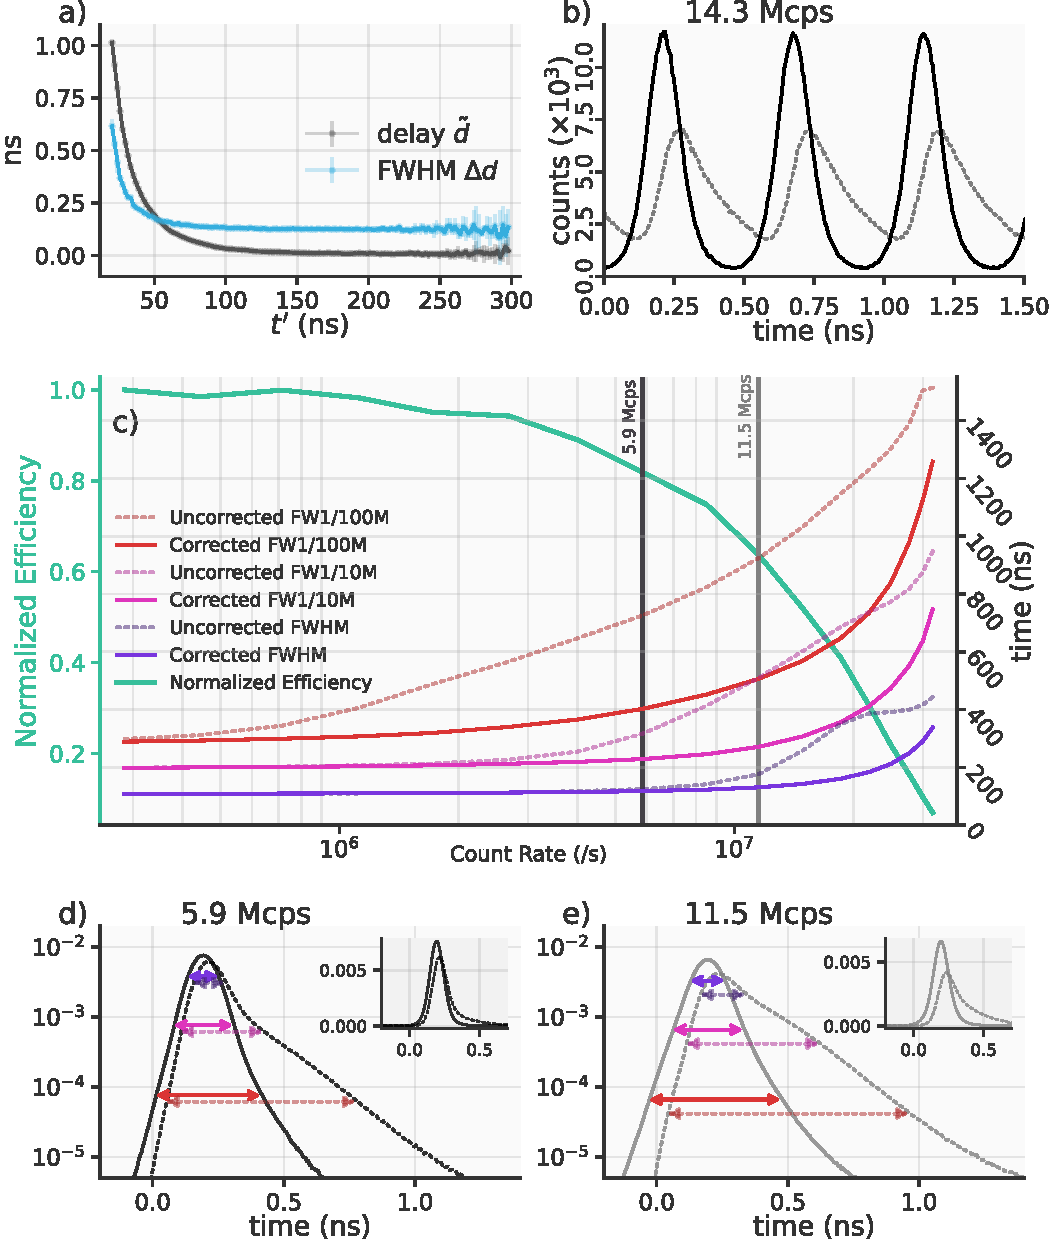
\includegraphics[width=0.7\textwidth,height=\textheight]{chapter_01/figs_01/Figure_Data_Sept_2022.pdf}
\caption[{A jitterate data figure.}]{\textbf{Figure Title.} And I think
the rest of this is the caption with (A), (B), and (C) callouts}
\label{fig:custom_figure}
\end{figure}
}

Finally, here's a png figure for testing

\hypertarget{fig:test_png_figure}{%
\begin{figure}
\centering
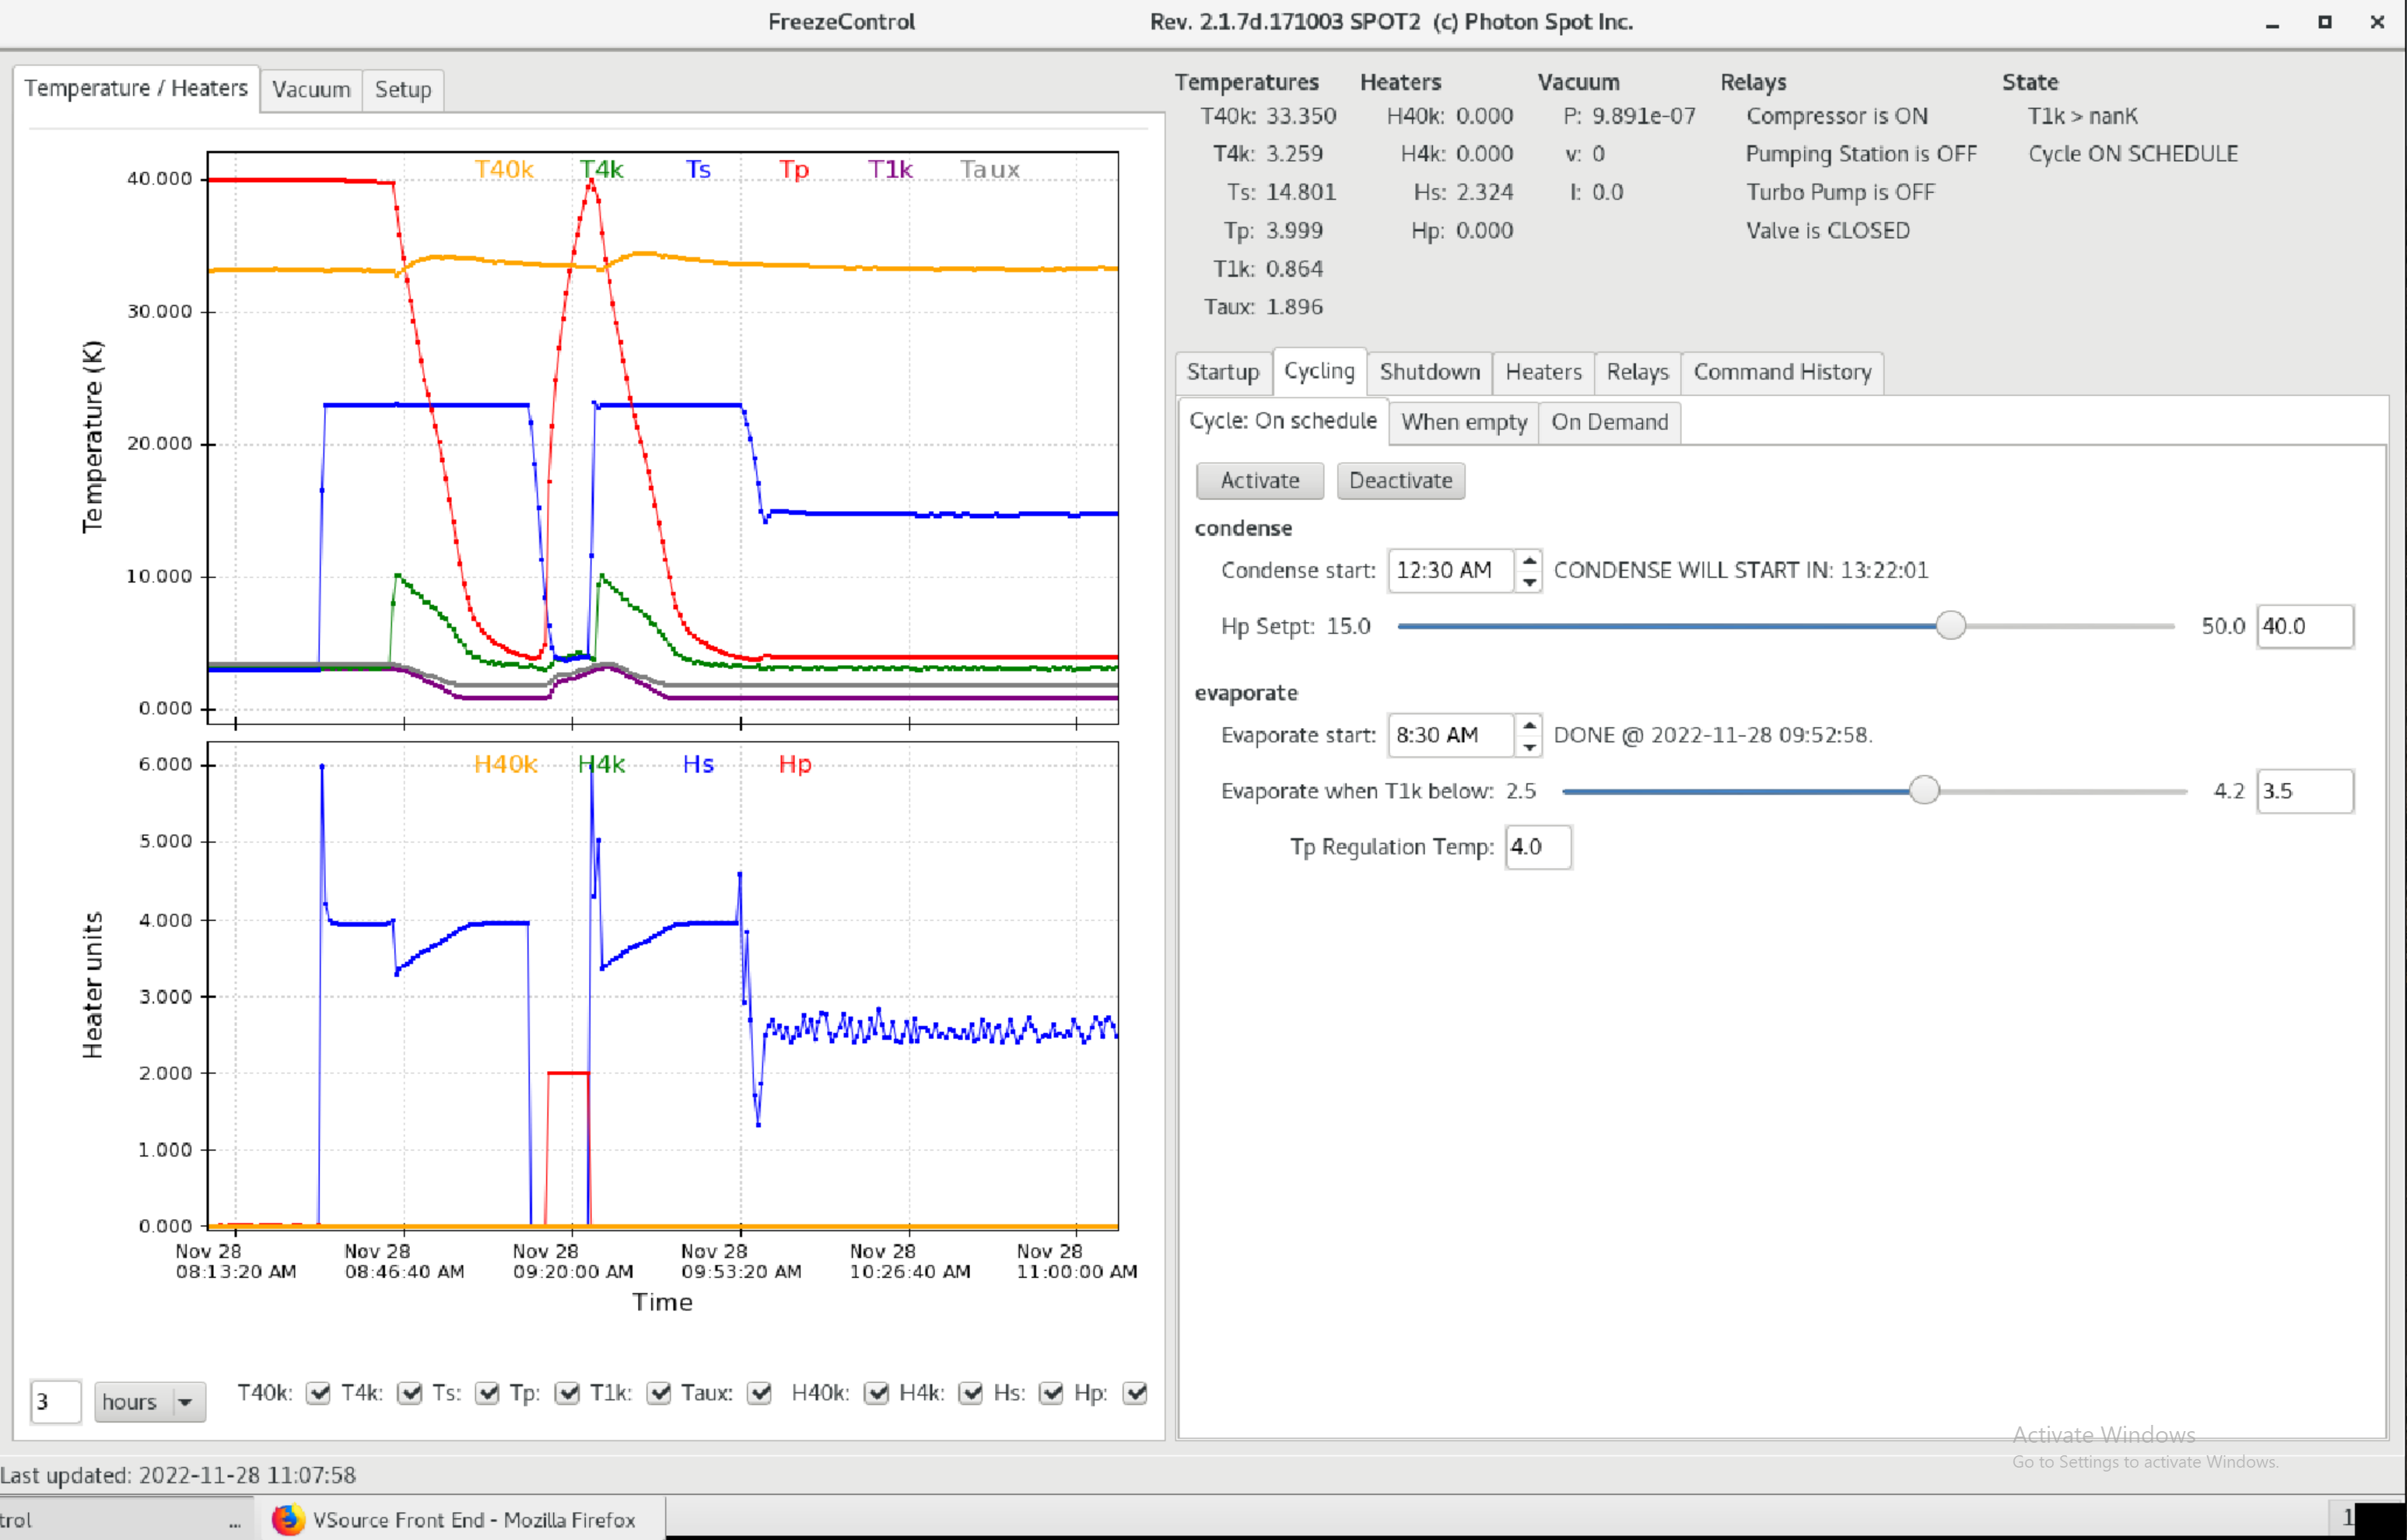
\includegraphics[width=0.7\textwidth,height=\textheight]{chapter_01/figs_01/fridge.png}
\caption[{A png figure.}]{\textbf{A test png figure.} And here is where
I'd put in more information about the png.}
\label{fig:test_png_figure}
\end{figure}
}

\hypertarget{high-rate-pulse-position-modulation}{%
\chapter{High Rate Pulse Position
Modulation}\label{high-rate-pulse-position-modulation}}

~~~~~~~~~~~~~~~~~~~~~~~~~~~~~~\includegraphics{chapter_groarse_grain.pdf}

\hypertarget{abstract-1}{%
\section{Abstract}\label{abstract-1}}

~~~~~ This study aimed to evaluate the feasibility of transmitting high
clock-rate pulse position modulated (PPM) data using a mode-locked laser
and receiving it with a low jitter superconducting nanowire
single-photon detector (SNSPD). The investigation was driven by recent
advancements in NbN SNSPDs, which have achieved a jitter as low as 50 ps
at the FW(1/100)M level, enabling the demonstration of PPM with 50 ps
slot widths and a 20 GHz clock. The aim was to increase the data rate by
a factor of 10, from 2 GHz to 20 GHz, in the next generation of the Deep
Space Optical Communication (DSOC) project.

During the course of this study, the focus shifted towards investigating
the impact of photon number resolution (PNR) on the low jitter detection
of optical pulses. PNR can have an unintended impact on the
demonstration of high-rate PPM, and therefore a thorough study of its
effects was deemed crucial. A novel PNR cancellation technique was
developed and applied to successfully demonstrate high-rate PPM. This
technique is considered essential for future low-jitter applications of
SNSPDs that exhibit photon-number effects.

\hypertarget{introduction-1}{%
\section{Introduction}\label{introduction-1}}

~~~~~ This study aimed to evaluate the feasibility of transmitting high
clock-rate pulse position modulated (PPM) data using a mode-locked laser
and receiving it with a low jitter superconducting nanowire
single-photon detector (SNSPD). The investigation was driven by recent
advancements in NbN SNSPDs, which have achieved a jitter as low as 50 ps
at the FW(1/100)M level, enabling the demonstration of PPM with 50 ps
slot widths and a 20 GHz clock. The aim was to increase the data rate by
a factor of 10, from 2 GHz to 20 GHz, in the next generation of the Deep
Space Optical Communication (DSOC) project.

During the course of this study, the focus shifted towards investigating
the impact of photon number resolution (PNR) on the low jitter detection
of optical pulses. PNR can have an unintended impact on the
demonstration of high-rate PPM, and therefore a thorough study of its
effects was deemed crucial. A novel PNR cancellation technique was
developed and applied to successfully demonstrate high-rate PPM. This
technique is considered essential for future low-jitter applications of
SNSPDs that exhibit photon-number effects.

\hypertarget{pulse-position-modulation-for-deep-space-communication}{%
\subsection{Pulse Position Modulation for Deep Space
Communication}\label{pulse-position-modulation-for-deep-space-communication}}

~~~~~ Deep Space Optical Communication has been a growing field of study
in recent years, as researchers look for ways to communicate with
spacecraft that are far away from Earth. In this article, we will focus
on the use of Pulse Position Modulation (PPM) for deep space optical
communication.

While other modulation techniques such as quadrature amplitude
modulation (QAM) have been used in the past, it has been shown that in
the photon-starved regime, PPM is the best approach for sending data.
This is because there is not enough light to measure the phase of the
signal.

PPM relies on sending one optical pulse carrying M bits of information
in one of \(2^M\) possible time slots. For M = 2, this corresponds to
sending an early pulse to represent a 0 bit and a late pulse to
represent a 1 bit.

The main challenge in deep space optical communication is the high loss
and distance that the link must traverse. This limits the communication
from the spacecraft, as it is limited by the power available on the
spacecraft. This means that the communication protocol is limited by the
number of bits that can be sent per unit of energy on the spacecraft,
also known as photon information efficiency or bits per photon.

For large M, PPM achieves high photon information efficiency, allowing
for the saving of power on the spacecraft and the sending of more
information with fewer photons. The existing deep space optical
communication project uses M up to \(2^8 = 256\), meaning that 8 bits of
data are carried in each optical pulse.

In this project, we aimed to demonstrate even higher photon information
efficiency by using M values up to 2048, or 11 bits of data per optical
pulse.

While the use of large M values increases photon information efficiency,
it also decreases the data rate of the system. This is because the
number of time bins needed per optical pulse scales exponentially with
the amount of data in each pulse. Therefore, for a given fixed clock
rate and time bin duration, the data rate decreases dramatically for
higher M values.

Using M values much larger than 11 is unlikely to be practical in future
deep space optical communication systems. However, the data rate of
these systems can be increased linearly by increasing the clock rate or
bin size of the experiment. This is possible with the use of low jitter
detection systems or low jitter superconducting nanowire single-photon
detectors (SNSPDs).

\hypertarget{development-of-a-modulation-source}{%
\subsection{Development of a modulation
source}\label{development-of-a-modulation-source}}

~~~~~ The communication signal on a spacecraft is generated by utilizing
a Continuous Wave (CW) seed laser that is carved by a fast intensity
modulator. The resulting low-power pulsed signal is then amplified by an
Erbium Doped Fiber Amplifier (EDFA) to increase its transmission power
to Earth. The majority of the power used by the spacecraft for
communication scales with the number of optical pulses due to the EDFA.

In our experiment, the 20 GHz repetition rate was limited by the jitter
of the Single-Photon Detectors (SNSPDs) that we intended to use. These
detectors have a Full Width at Half Maximum (FW(1/100)M) jitter of
approximately 50 ps. To ensure that the response function of the entire
experiment had jitter of around 50 ps FW(1/100)M, we needed to build a
Pulsed Phase Modulation (PPM) source with ultra-short optical pulses.

Carving a CW laser with our system would have introduced excessive
timing uncertainty due to the limited ability of even the fastest
lithium niobate intensity modulators to carve pulses with widths below
20 ps. The added jitter from modulated CW pulses, combined with the
jitter of the detectors, would have exceeded the 20 GHz/50 ps slot width
requirement.

Therefore, we chose to carve pulses from a mode-locked laser. This
approach allows for extremely short pulses in time, with the modulators
responsible for sufficiently reducing any surrounding unwanted pulses.
The temporal width of the modulator pulse response must be extremely
short and able to modulate from `off' to `on' within a time frame of the
order of the 50 ps bin width.

\hypertarget{initial-tests-and-performance}{%
\section{Initial tests and
performance}\label{initial-tests-and-performance}}

\emph{This is where I will describe the initial problems with the first
iteration of the experiment, using one modulator and not taking into
account PNR effects.}

\hypertarget{synchronization-with-a-software-phase-locked-loop-pll}{%
\section{Synchronization with a Software Phase Locked Loop
(PLL)}\label{synchronization-with-a-software-phase-locked-loop-pll}}

\textbf{Todo} \emph{This will be the first place in the thesis that I
introduce the use of my software based phase locked loop (PLL). The
software PLL has been useful in several later projects. I will either
fully explain the PLL here, or I will only introduce and motivate it
here. And a full description will go in an appendix. } 1. For sending
many PPM symbols, I needed a synchronization clock that was (A) always
running, and (B) extremely low jitter. 2. Sending an output from the AWG
to the Swabian timetagger in another room resulted in a less-than-ideal
clock source. The signal was low amplitude, and triggering on it's
rising edge did not make for a very low jitter clock signal. 3. I had
some sense that that should be a way of `averaging' past clock cycles in
some way to cancel jitter. After some research and failed tests toward
developing my own averaging method, I learned a software based Phase
Locked Loop is just what I needed. 4. Initial version was adapted from a
Matlab code on the Phase Locked Loop wikipedia page. That code was
written for a sampled sign wave, but I adapted to take in just one data
point per period. For our non-coherent and time-resolved types of
measurements with SNSPDs, we typically only have clocks of this type.
Where the clock is expressed by some type of optical or RF pulse that
arrives on a regular period. 5. More recently Rahaf Youssef and I have
worked on updating our software PLL tools so that its easier to
understand and reason about, and easier to lock to a given signal.

\hypertarget{pnr-characterization}{%
\section{PNR Characterization}\label{pnr-characterization}}

\textbf{Todo:} - {[} {]} This is where I'll show the first scans of the
rising edge of the NbN nanowire pulse - {[} {]} Convey how triggering at
any level results in weird multi-modal histograms because of the PNR
effect - {[} {]} State that initially the idea was to fully characterize
the PNR component, as in identify each pulse as \(|1\rangle\),
\(|2\rangle\), \(|3\rangle\) or so on. Then, apply a fixed correction
value to the arrival time the cancel out the effect - {[} {]} That
approach didn't work out because in the 3 photons per pulse range, the
true photon number gets harder to identify. It's not clear if a pulse is
a \(|3\rangle\) or a \(|4\rangle\), and the arrival time of the optical
pulse is correspondingly uncertain.

\hypertarget{time-walk-and-jitter-correction}{%
\chapter{Time Walk and Jitter
Correction}\label{time-walk-and-jitter-correction}}

~~~~~~~~~\includegraphics{chapter_pdutant.pdf}

A version of this chapter originally appeared as Chure, G, Razo-Mejia,
M., Belliveau, N.M., Kaczmarek, Zofii A., Einav, T., Barnes, Stephanie
L., Lewis, M., and Phillips, R. (2019). Predictive shifts in free energy
couple mutations to their phenotypic consequences. Proceedings of the
National Academies of Sciences 116(37) DOI:
https://doi.org/10.1073/pnas.1907869116. G.C., M.R.M, N.M.B., Z.A.K.,
and S.L.B designed the experiments and collected and analyzed data. G.C.
developed the theoretical treatment of free energy shifts. G.C., M.R.M,
N.M.B., Z.A.K., T.E., S.L.B., and R.P. designed the research project.
G.C. and R.P. wrote the paper. M.L. provided guidance and advice.

\hypertarget{abstract-2}{%
\section{Abstract}\label{abstract-2}}

This is an overview of the time walk and jitter correction section. More
details to come.

\hypertarget{introduction-2}{%
\section{Introduction}\label{introduction-2}}

~~~~~ To be written.

\hypertarget{the-peacoq-detector-and-higher-order-correction-methods}{%
\section{The Peacoq Detector, and Higher Order Correction
Methods}\label{the-peacoq-detector-and-higher-order-correction-methods}}

\hypertarget{outlook-towards-high-rate-pnr-and-time-walk-correction}{%
\section{Outlook: Towards High Rate PNR and Time Walk
Correction}\label{outlook-towards-high-rate-pnr-and-time-walk-correction}}

\hypertarget{high-rate-entanglement-generation}{%
\chapter{High Rate Entanglement
Generation}\label{high-rate-entanglement-generation}}

~~~~~~~~~~~~~~~~~~~~~~~~~~~~~~~~~~~~\includegraphics{chapter_oghysiology.pdf}

A version of this chapter is currently under review. A preprint is
released as Chure, G, Kaczmarek, Z. A., and Phillips, R. Physiological
adaptability and parametric versatility in a simple genetic circuit.
bioRxiv 2019. DOI: 10.1101/2019.12.19.878462. G.C. and R.P. designed
experiments and developed theoretical models. G.C. and Z.A.K. collected
and analyzed data. G.C. and R.P. wrote the paper.

\hypertarget{abstract-3}{%
\section{Abstract}\label{abstract-3}}

\hypertarget{introduction-3}{%
\section{Introduction}\label{introduction-3}}

Cellular physiology is inextricably tied to the extracellular
environment. Fluctuations in nutrient availability and variations in
temperature, for example, can drastically modulate the cell's growth
rate, which is often used as a measure of the evolutionary fitness
\autocite{schaechter1958}. In response to such environmental insults,
cells have evolved myriad clever mechanisms by which they can adapt to
their changing surroundings, many of which involve restructuring their
proteome such that critical processes (i.e.~protein translation) are
allocated the necessary resources. Recent work exploring this level of
adaptation using mass spectrometry, ribosomal profiling, and RNA
sequencing have revealed that various classes of genes (termed
``sectors'') are tuned such that the protein mass fraction of the
translational machinery is prioritized over the metabolic and catabolic
machinery in nutrient replete environments
\autocite{scott2014,klumpp2014,hui2015,schmidt2016,li2014}. This drastic
reorganization is mediated by the regulation of gene expression, relying
on the concerted action of myriad transcription factors. Notably, each
gene in isolation is regulated by only one or a few components
\autocite{gama-castro2016}. The most common regulatory architecture in
\emph{Escherichia coli} is the simple repression motif in which a
transcriptional repressor binds to a single site in the promoter region,
occluding binding of an RNA polymerase
\autocite{rydenfelt2014,phillips2019}. The simple activation
architecture, in which the simultaneous binding of an activator and an
RNA polymerase amplifies gene expression, is another common mode of
regulation. Combinatorial regulation such as dual repression, dual
activation, or combined activation and repression can also be found
throughout the genome, albeit with lower frequency
\autocite{phillips2019}. The ubiquity of the simple repression and
simple activation motifs illustrate that, for many genes, the complex
systems-level response to a physiological perturbation boils down the
binding and unbinding of a single regulator to its cognate binding
sites.

~~~~~Despite our knowledge of these modes of regulation, there remains a
large disconnect between concrete, physical models of their behavior and
experimental validation. The simple repression motif is perhaps the most
thoroughly explored theoretically and experimentally
\autocite{phillips2019} where equilibrium thermodynamic
\autocite{garcia2011,garcia2012,brewster2014,razo-mejia2018,barnes2019}
and kinetic \autocite{jones2014,ko1991,kepler2001,michel2010} models
have been shown to accurately predict the level of gene expression in a
variety of contexts. While these experiments involved variations of
repressor copy number, operator sequence, concentration of an external
inducer, and amino acid substitutions, none have explored how the
physiological state of the cell as governed by external factors
influences gene expression. This is arguably one of the most critical
variables one can experimentally tune to understand the roles these
regulatory architectures play in cellular physiology writ large.

~~~~~In this work, we interrogate the adaptability of a simple genetic
circuit to various physiological stressors, namely carbon source quality
and growth temperature. Following the aforementioned thermodynamic
models, we build upon this theory-experiment dialogue by using
environmental conditions as an experimentally tunable variable and
determine their influence on various biophysical parameters.
Specifically, we use physiological stressors to tune the growth rate.
One mechanism by which we modulate the growth rate is by exchanging
glucose in the growth medium for the poorer carbon sources glycerol and
acetate, which decrease the growth rate by a factor of \(\approx\) 1.5
and \(\approx\) 4 compared to glucose, respectively. We hypothesize that
different carbon sources should, if anything, only modulate the
repressor copy number seeing as the relationship between growth rate and
total protein content has been rigorously quantified
\autocite{schaechter1958,schmidt2016,li2014,jun2018}. Using single-cell
time-lapse fluorescence microscopy, we directly measure the copy number
of the repressor in each condition. Under a simple hypothesis, all other
parameters should be unperturbed, and we can thus rely on previously
determined values to make parameter-free predictions of the fold-change
in gene expression.

~~~~~Despite the decrease in growth rate, both the fold-change in gene
expression and the repressor copy number remains largely unaffected. We
confirm this is the case by examining how the effective free energy of
the system changes between carbon sources, a method we have used
previously to elucidate parametric changes due to mutations within a
transcription factor \autocite{chure2019} and has been extensively
discussed in Chapter 3. This illustrates that the energetic parameters
defining the fraction of active repressors and their affinity for the
DNA are ignorant of the carbon-dependent physiological states of the
cell. Thus, in this context, the values of the biophysical parameters
determined in one condition can be used to draw predictions in others.

~~~~~We then examine how variations in temperature influence the
transcriptional output. Unlike in the case of carbon source variation,
temperature dependence is explicit in our model: the repressor-DNA
binding energy and the energetic difference between the active and
inactive states of the repressor are scaled to the thermal energy of the
system at 37\(^\circ\) C. This is defined via the Boltzmann distribution
which states that the probability of a state \(p_{state}\) is related to
the energy of that state \(\varepsilon_{state}\) as
\begin{equation}\protect\hypertarget{eq:boltz}{}{
p_{state} \propto e^{-\varepsilon_{state} / k_BT},
}\label{eq:boltz}\end{equation} where \(k_B\) is the Boltzmann constant
and \(T\) is the temperature of the system. Given knowledge of \(T\) for
a particular experiment, we can easily draw predictions of the
fold-change in gene expression. However, we find that the fold-change in
gene expression is inconsistent with this simple model, revealing an
incomplete description of the energetics. We then examine how entropic
effects neglected in the initial estimation of the energetic parameters
may play an important role; a hypothesis that is supported when we
examine the change in the effective free energy.

~~~~~

\hypertarget{appendix-1}{%
\chapter{Appendix 1}\label{appendix-1}}

~~~~~~~~~~~~~\includegraphics{chapter_stoming_storm.pdf}

\hypertarget{abstract-4}{%
\section{Abstract}\label{abstract-4}}

This is an overview of the appendix section. More details to come.

\hypertarget{software-systems-and-operation}{%
\section{Software Systems and
Operation}\label{software-systems-and-operation}}

\hypertarget{aph-138-homework-assignment}{%
\section{Aph 138 Homework
Assignment}\label{aph-138-homework-assignment}}

{\color{midnightblue} Contact
\href{mailto:andrewstermueller@gmail.com}{Andrew Mueller} with any
questions about the homework or solution manual. The solutions to some
sections specify finer-grained point values when there are multiple
answers per section. As the grader, feel free to use these or not. }.

\hypertarget{free-space-coupling-with-low-dark-counts-50-points}{%
\subsection{1. Free space coupling with low dark counts {[}50
points{]}}\label{free-space-coupling-with-low-dark-counts-50-points}}

An experimental apparatus emits a collimated beam of
\(1550~\mathrm{nm}\) photons with gaussian beam waist
\(w_0 = 3~\mathrm{mm}\). You wish to focus the beam onto an SNSPD
directly through a window in a cryostat.

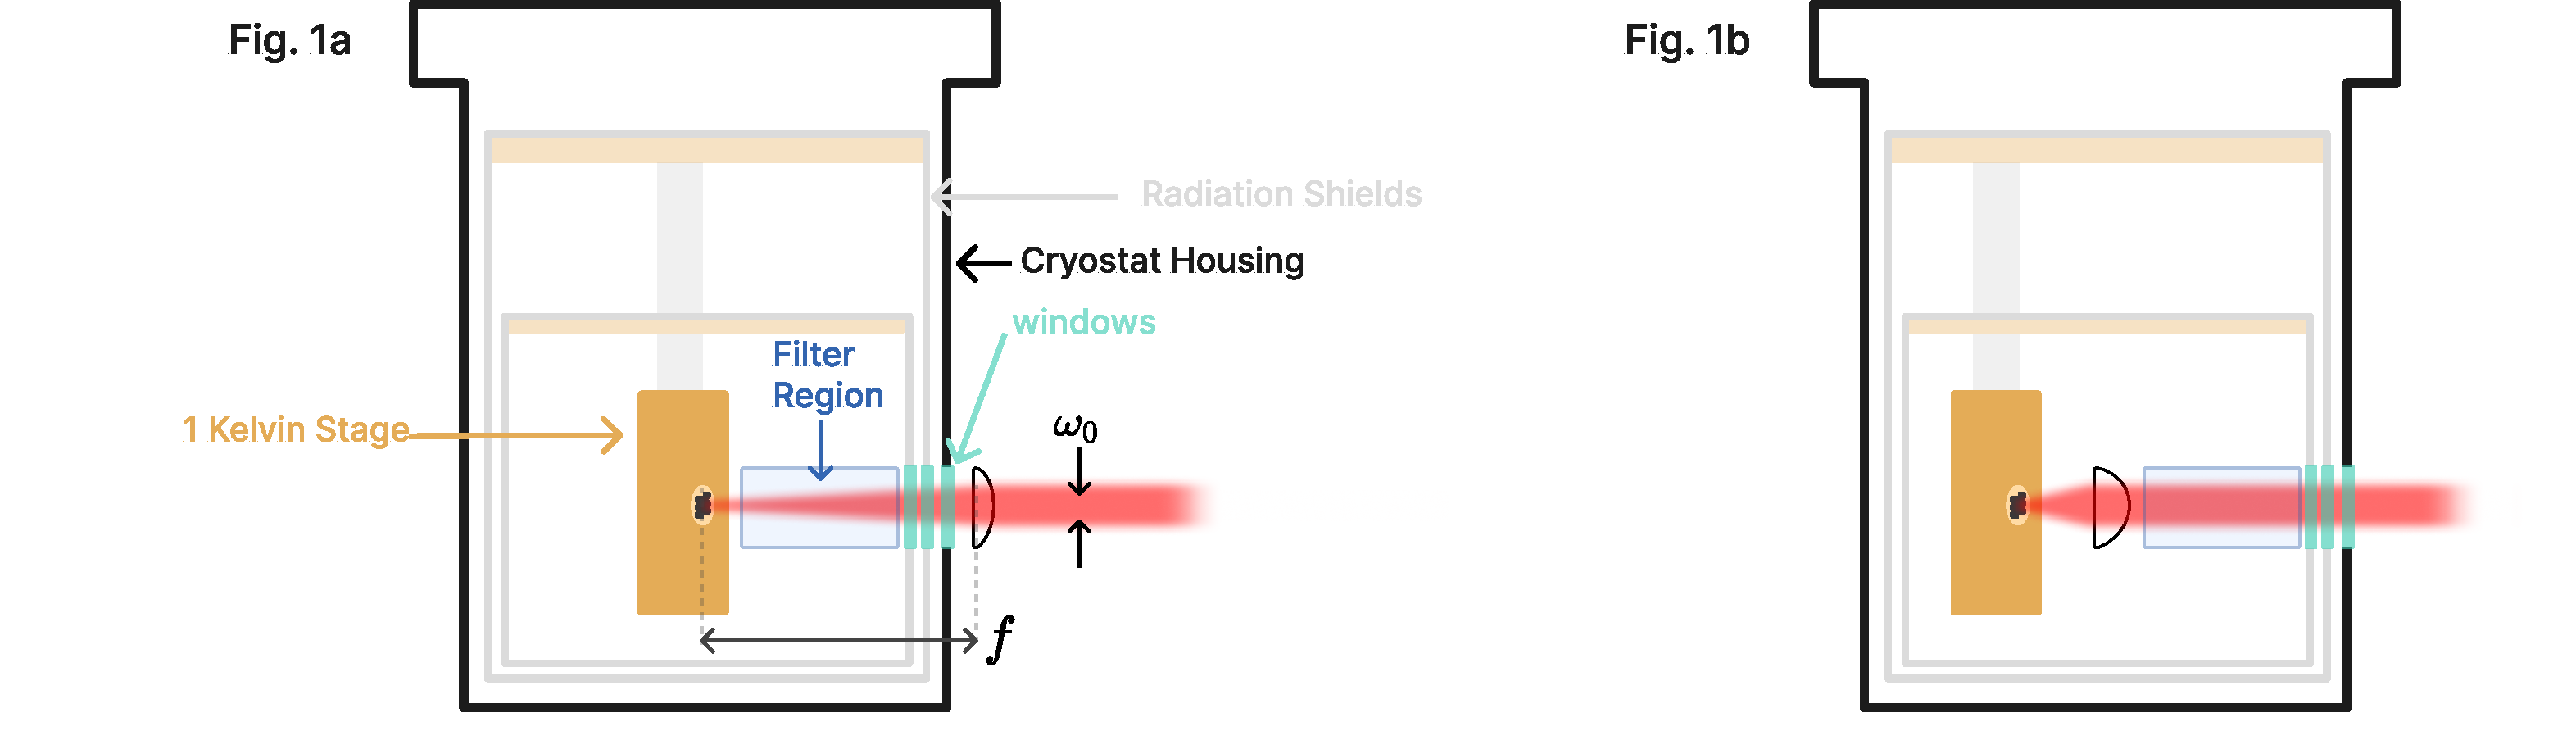
\includegraphics{chapter_05/figs_05/fig1_light.pdf}\includegraphics{chapter_05/figs_05/fig1_dark.pdf}

\printbibliography
\end{document}
